\section{Microscopic Sources of Exotic Stiffness}

\subsection{Review}
Last time, we tried to constrain the stiffness tensor:
\begin{equation}
    \sigma^\alpha = K^{\alpha\beta}u^\beta
\end{equation}

Assuming isotropy, the subspaces of scalars and vectors could not be connected (so the off diagonal blocks vanish), and assuming frame invariance, rotations cannot generate any stresses, so:
\begin{equation}
    \m{\text{P} \\ \text{T} \\ \text{SS1} \\ \text{SS2}} = \m{\cdot & 0 & 0 & 0 \\ \cdot & 0 & 0 & 0 \\ 0 & 0 & \cdot & \cdot \\ 0 & 0 & \cdot & \cdot}\m{\text{D} \\ \text{R} \\ \text{S1} \\ \text{S2}}
\end{equation}
Isotropy further contains that the lower diagonals are the same and lower off diagonals are the same, so the most general form of the tensor is:
\begin{equation}\label{eq:macroscopic}
    \m{\text{P} \\ \text{T} \\ \text{SS1} \\ \text{SS2}} = \m{B & 0 & 0 & 0 \\ A & 0 & 0 & 0 \\ 0 & 0 & G & -K^0 \\ 0 & 0 & +K^0 & G}\m{\text{D} \\ \text{R} \\ \text{S1} \\ \text{S2}}
\end{equation}
Important point - the existence of the odd elastic moduli $K^0$ implies two things. First, the structure of the theory is non-variational; we can go around quasi-statically in the space of strains, and we find the work is nonzero:
\begin{equation}
    W = \oint \sigma_{ij}du_{ij}\neq 0
\end{equation}
This tells us that there is a chirality in the material (this was also manifest from the fact that - if $G = 0$, then the part of the stiffness matrix acting on the shear subspace looks like $K^0\e$). Another clear manifestation of chirality is if $A \neq 0$, in which case we can have torques (note - no angular momentum conservation!) as a result of dilations.

\subsection{Non-reciprocal gadget and constructions}
This is an example of a $K^0 \neq 0, A = 0$ system from a recent Nature paper \texttt{Veenstra, Scheibner, Brandenbourger, Binysh, Souslov, Vitelli, Coulais. \emph{Nature} (2025)}. As warm-up, consider the following spring system:

\begin{center}
    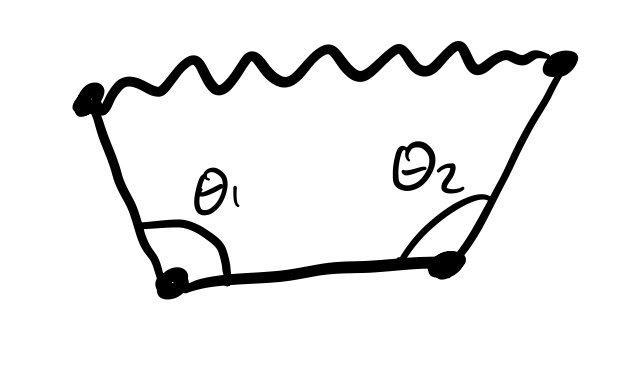
\includegraphics[scale=0.35]{Lectures/Images/lec3-gadgetwithspring.png}
\end{center}

If we have a bond-bending interaction, we have a bond-bending stiffness:
\begin{equation}
    \m{\tau_1 \\ \tau_2} = \m{-\kappa & \kappa^s \\ \kappa^s & -\kappa}\m{\delta\theta_1 \\ \delta\theta_2}
\end{equation}
where the diagonals come from the bond-bending, and the off-diagonals (symmetric!) come from the coupling spring. For this system:
\begin{equation}
    \nabla \times \gv{\tau} = \v{0}
\end{equation}
but we can introduce batteries/motors to break this symmetry. If Maxwell-Betti reciprocity is obeyed, then pushing one side of the object should repel the other symmetrically. But we can introduce motors to make this building block non-reciprocal; pressing on the left side the right side repels, pressing on the right side the left side \emph{attracts}.
\begin{center}
    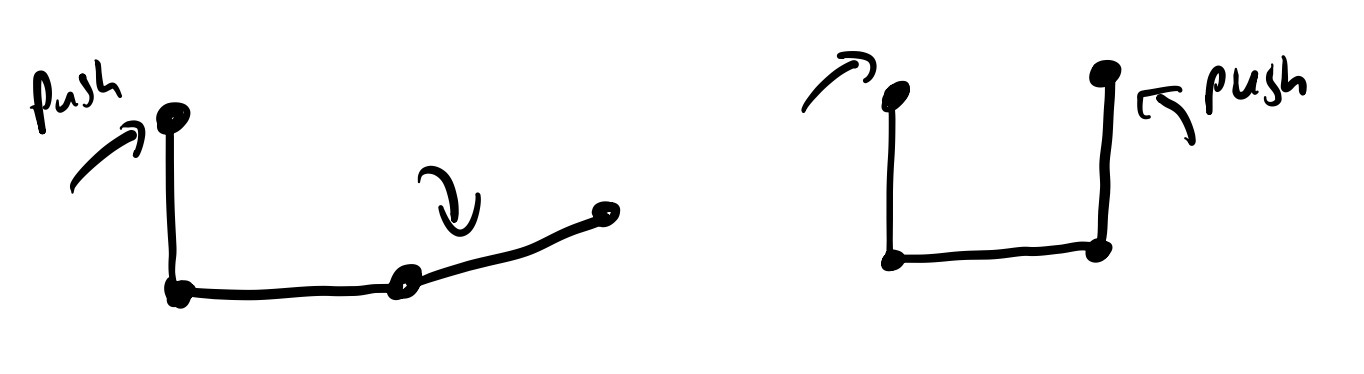
\includegraphics[scale=0.35]{Lectures/Images/lec3-nonreciprocalgadget.png}
\end{center}
This means that we have a stiffness tensor of the form:
\begin{equation}\label{eq:microscopic}
    \m{\tau_1 \\ \tau_2} = \m{-\kappa & -\kappa^a \\ \kappa^a & -\kappa}\m{\delta\theta_1 \\ \delta\theta_2}
\end{equation}

A technical comment - notice that the interaction we've written above is a striking example of a non-pairwise interaction. The torque at point 1 doesn't just depend on the pair of rods eminating out of it, but also from the other components of the system.

What is the physical consequence of this non-reciprocal interaction? Now, we can go through a cycle and generate non-zero work. If we make a ring of these objects - with the motors off, the system jiggles a bit before being slowed to rest with friction. With the motors on, we perturb the medium and in trying to undo the deformation/get back to the starting point the motors can induce energies into the system and the system can keep jiggling forever (using the energy provided by the external motors).

If we think about the dynamics, we have:
\begin{equation}
    \m{I\delta \ddot{\theta}_1 \\ I\delta \ddot{\theta}_2} = \m{-\kappa & -\kappa^a \\ \kappa^a & \kappa}\m{\delta \theta_1 \\ \delta\theta_2}
\end{equation}
If we diagonalize to find the normal frequencies, we have:
\begin{equation}
    \omega^2 = \frac{\kappa}{I} \pm i\frac{\kappa^a}{I}
\end{equation}
The first term makes total sense - this is what we have for just a regular spring system that you've seen many times before in classical mechanics. But the antisymmetric term produces an imaginary component to $\omega^2$! This means that (in the absence of nonlinearities - we have assumed linear response for this whole discussion) we have unbounded growth/amplification of the motion! Of course building this gadget in real life we do in fact have nonlinearities - when the angles become large the components of the gadget can touch - which prevents unbounded growth.

Now, we can take our object - where the antisymmetric $\kappa^a$ breaks the chiral symmetry - and map out the dynamics in strain space (with the two shears being the two axes). The system can exhibit chaotic behaviour!

Let us ``rediscover'' the wheel (again, still composed of the the gadget). Original conception of a wheel has a circular, fixed shape which moves via force supplied to it from axle (via animal, motor etc.) But our new wheel is adaptive, and moves via deformations. It can come across a rough uphill landscape and use the deformations caused by the rough landscape to travel through it! In fact we can make the problem even harder - we can make a landscape of granular uphill matter, and our sophisticated wheel can still go up it (we can also flip the sign of $\kappa^a$ - we are allowed to pick/tune whatever sign for these - and it can travel the other way).

We can also build up a crystal out of this gadget by tiling. We can throw a projectile onto the crystal, which is then ejected back upwards at an angle (the angle/asymmetric response is expected! The medium is chiral. Again, we can flip the angle by flipping the sign of $\kappa^a$).

Motivating a homework problem you will do - there is a microscopic law Eq. \eqref{eq:microscopic} and the macroscopic/continuum description Eq. \eqref{eq:macroscopic}. Without calculation, we can deduce $K^0 \sim \kappa^a$ and $G \sim \kappa$. We can do a more detailed derivation and derive the macroscopic dependence on the microscopic parameters (and then check that this dependence works out in experiment)! In your homework, you will just take a normal (not odd!) hexagonal microscopic lattice, and see how the macroscopic properties/parameters and their dependencies emerge.

\subsection{Microscopic source of $A$}

If we have a central force, we can generically write things as a gradient of a potential. We introduce non-conservative forces in terms of a non-central part. Consider the spring:

\begin{center}
    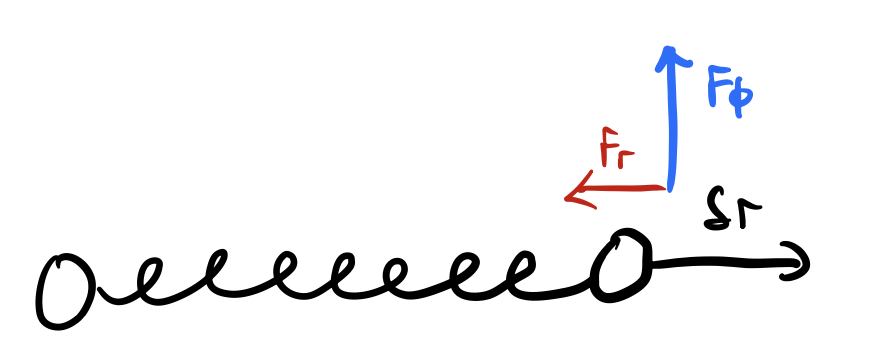
\includegraphics[scale=0.35]{Lectures/Images/lec3-noncentralspring.png}
\end{center}

\begin{equation}
    \v{F} = -(\kappa\hat{\v{r}} + \kappa^a\hat{\gv{\phi}})\delta r
\end{equation}
Or as a matrix equation:
\begin{equation}
    \m{F_r \\ F_\phi} = \m{-\kappa & 0 \\ -\kappa^a & 0}
\end{equation}
Notice again the crucial point - the off-diagonals are \emph{not} equal. This implies that:
\begin{equation}
    \oint \v{F} \cdot d\v{l} \propto \kappa^a
\end{equation}
(and does not vanish). The central part does not contribute to the net work as to the central part we can always prescribe a potential. Generally here, $\v{F} \neq -\nabla U$ so long as $\kappa^a \neq 0$. If we built up a lattice/continuum out of this microscopic piece, we could derive how the $A$ modulus emerges from the nonzero $\kappa^a$.

Let us consider a simple exercise - let's derive the work done in a cycle.

\begin{center}
    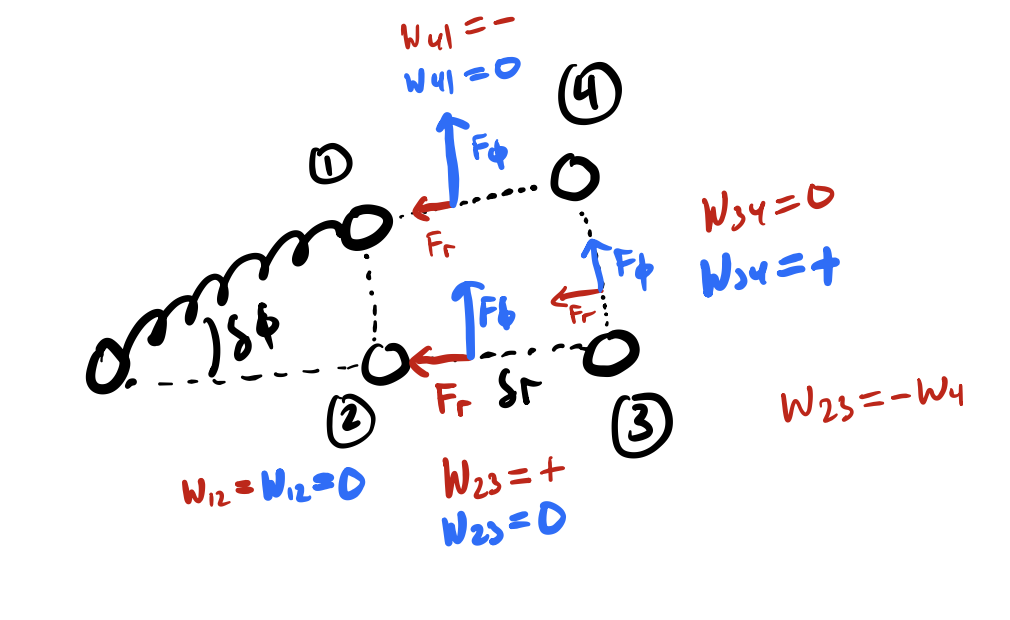
\includegraphics[scale=0.5]{Lectures/Images/lec3-noncentralspringwork.png}
\end{center}

\begin{itemize}
    \item From 1 to 2, there is no force and hence no work done.
    \item From 2 to 3, the direction of motion is radial, so only the radial component of the force contributes (positive) work.
    \item From 3 to 4, the direction of motion is tangential, so the tangential component of the force picks up (positive) work.
    \item From 4 to 1, the direction of motion is radial, so the radial component of the force contributes (negative) work. This work is equal and opposite to the work in step 2$\to$3.
\end{itemize}

Thus only surviving term is $W_{34}$ arising from $F_\phi$, which we can calculate to be:
\begin{equation}
    \oint \v{F} \cdot d\v{l} = W_{34} = F_\phi dl = \kappa^a \delta r (r + \delta r)\delta \phi \approx \kappa^a (r\delta \phi)\delta r = \kappa^a \cdot \text{Area}
\end{equation}

So in the harmonic approximation, with:
\begin{equation}
    F''(r) = F''(a) - \kappa(r - a), \quad F_\perp \approx F^\perp(a) - \kappa^a(r - a)
\end{equation}
we can derive the bulk and shear moduli:
\begin{equation}
    B = \frac{\sqrt{3}}{2}\left(\kappa + \frac{F''(a)}{a}\right), \quad G = \frac{\sqrt{3}}{4}\left(\kappa - 3\frac{F''(a)}{a}\right)
\end{equation}
as well as the $K^0/A$ moduli:
\begin{equation}
    A = -\frac{\sqrt{3}}{2}\left(\kappa^a - \frac{F^\perp(a)}{a}\right), \quad K^0 = \frac{\sqrt{3}}{4}\left(\kappa^a - 3\frac{F^\perp(a)}{a}\right)
\end{equation}
note that the precise dependence depends on not just the force mechanism but also the layout of the lattice (e.g. will change with hexagonal, square etc.). If we did a similar derivation with the non-reciprocal robot gadget, we could also derive a macro-from-micro result from above (see the paper!), with $A = 0$ and $K^0 \neq 0$.

\subsection{Other contemporary experiments}

There have been a number of recent experiments that measure interesting non-central crystals. For example colloidal spinners in a magnetic field that form odd elastic crystals \texttt{Bililign, Usabiaga, Ganan, Poncet, Soni, Magkiriadou, Shelley, Bartolo, Irvine. \emph{Nature} (2022)} or crystal formation in biological platforms \texttt{Tan, Mietke, Higinbotha, Li, Chen, Foster, Gokhale, Dunkel, Fakhri. \emph{Nature} (2022)}.

In such non-central crystals, there is the potential to measure lubrication forces:

\begin{center}
    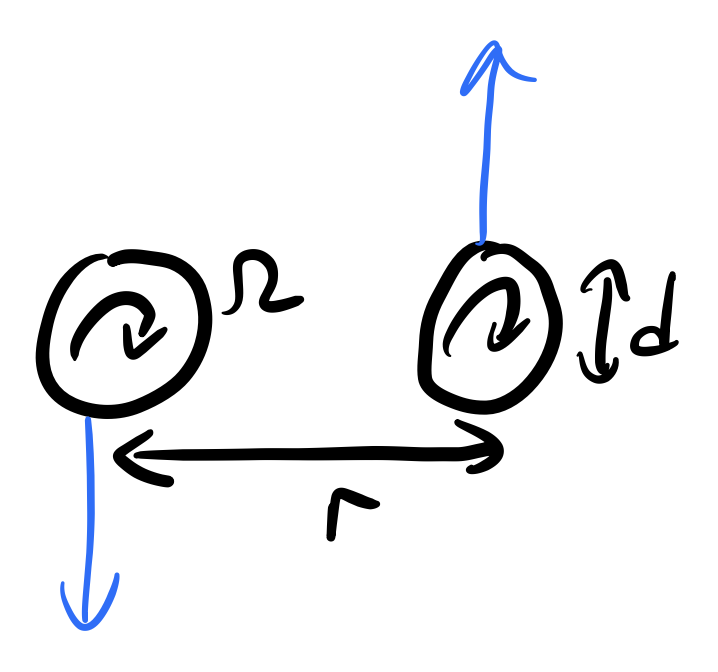
\includegraphics[scale=0.35]{Lectures/Images/lec3-lubricationforces.png}
\end{center}

where:
\begin{equation}
    F^\perp \propto \Omega \log\left(\frac{r - d}{d}\right)
\end{equation}

Next time - we will take the macroscopic theory, and study the stability of the lattice, as well as excitations (sound modes) in it. These have been concretely measured in robotic platform, and allegedly in the biological platform above (and perhaps possible to measure it in the colloidal spinner crystal?) however in the latter two cases the micro-to-macro correspondence is much well less understood.